\chapter{Pengujian dan Eksperimen}
\label{chap:testing}

\section{Skenario Pengujian Eksperimental}
\label{sec:exp-scenario}
Eksperimen dilakukan dengan menggunakan spesifikasi komputer sebagai berikut:

\begin{enumerate}
	\item Tipe \textit{processor}: Intel(R) Core(TM) i7-4720HQ CPU @2.60GHz
	\item Memori: 12288MB RAM
	\item Sistem operasi: Windows 10 Pro 64-bit (10.0, Build 17763)
\end{enumerate}

Pada suatu penelitian, ada beberapa jenis variabel yang diteliti di antaranya variabel bebas, variabel terikat, dan variabel kontrol. Pada penelitian ini, pengujian eksperimental dilakukan dengan tujuan untuk mengetahui hubungan antara parameter masukan dengan waktu dan hasil pengelompokan. Oleh karena itu, variabel bebas dari penelitian ini merupakan variabel yang menjadi parameter masukan yang terdapat pada antarmuka pengguna (Subbab \ref{sec:guidesign}). Namun, tidak semua parameter masukan yang terdapat pada antarmuka pengguna menjadi variabel bebas. Parameter masukan yang merupakan variabel bebas pada penelitian ini di antaranya adalah:

\begin{enumerate}
	\item Banyaknya populasi \\
	Jumlah individu yang dibentuk dalam proses pengelompokan menggunakan algoritma genetika.
	\item Metode pembobotan \\
	Metode penghitungan bobot suatu \textit{term} dalam vektor. Dalam penelitian ini digunakan dua metode yaitu bobot TF-IDF dan bobot frekuensi.
	\item Probabilitas mutasi \\
	Probabilitas terjadinya mutasi pada saat proses pembentukan keturunan dalam algoritma genetika.
	\item Individu elitisme \\
	Jumlah individu dengan \textit{fitness} terbaik yang langsung masuk ke generasi selanjutnya.
\end{enumerate}

Selain variabel bebas, terdapat juga variabel kontrol yang merupakan parameter masukan pada antarmuka pengguna. Variabel kontrol dalam penelitian ini adalah sebagai berikut:

\begin{itemize}
	\item Banyaknya \textit{cluster} \\
	Banyaknya cluster yang ingin dibentuk pada saat proses pengelompokan.
	\item Maksimum iterasi \\
	Batas maksimum iterasi yang dapat dilakukan selama proses pengelompokan dokumen.
	\item Banyaknya generasi konvergen \\
	Banyaknya generasi terakhir yang dilihat selisih nilai \textit{fitness}-nya.
	\item Batas konvergen \\
	Batas selisih nilai \textit{fitness} supaya dianggap memiliki nilai \textit{fitness} sama.
\end{itemize}

Variabel banyaknya \textit{cluster} dijadikan variabel kontrol karena nilai dari variabel ini harus disesuaikan dengan banyaknya topik pada \textit{dataset} (Subbab \ref{sec:dataset}) untuk mendapatkan hasil yang maksimal. Variabel maksimum iterasi juga merupakan variabel kontrol untuk menjaga agar proses pengelompokan tidak menjadi sangat lama karena terlalu banyak iterasi yang terjadi. Sama halnya untuk variabel banyaknya generasi konvergen dan batas konvergen, kedua variabel ini juga dapat menjaga agar iterasi yang terjadi tidak terlalu banyak sehingga menghabiskan waktu yang lebih banyak. Variabel terikat dalam penelitian ini adalah sebagai berikut:

\begin{itemize}
	\item Waktu \\
	Waktu yang diperlukan untuk mengelompokkan data.
	\item Nilai \textit{intracluster} \\
	Jumlah \textit{similarity} antara setiap dokumen ke masing-masing \textit{centroid}.
	\item Banyak iterasi \\
	Jumlah iterasi yang dilakukan selama proses pengelompokan.
	\item Nilai \textit{purity} \\
	Nilai yang menunjukkan akurasi dari pengelompokan (Subbab \ref{sec:purity}).
\end{itemize}

Keempat variabel terikat ini merupakan variabel yang dipengaruhi oleh berubahnya variabel bebas. Dalam penelitian ini hanya ada empat aspek yang diperhatikan yaitu waktu, nilai \textit{intracluster}, banyak iterasi, dan nilai \textit{purity}. Oleh karena itu, dibuat suatu skenario pengujian eksperimental untuk mengetahui pengaruh variabel bebas terhadap variabel terikat. Variasi nilai dari variabel bebas ditunjukkan dalam Tabel \ref{tbl:testScenario}.

\begin{table}[H]
	\centering
	\caption{Variasi nilai variabel bebas}
	\begin{tabular}{|l|l|}
		\hline
		Variabel Bebas                       & Variasi   \\ \hline
		\multirow{3}{*}{Banyaknya Populasi}  & 50        \\ \cline{2-2} 
		                                     & 100       \\ \cline{2-2} 
		                                     & 150       \\ \hline
		\multirow{2}{*}{Metode Pembobotan}   & TF-IDF    \\ \cline{2-2} 
		                                     & Frekuensi \\ \hline
		\multirow{3}{*}{Probabilitas Mutasi} & 0         \\ \cline{2-2} 
		                                     & 0.05      \\ \cline{2-2} 
		                                     & 0.25      \\ \hline
		\multirow{3}{*}{Individu Elitisme}   & 0         \\ \cline{2-2} 
 		                                     & 1         \\ \cline{2-2} 
		                                     & 5         \\ \hline
\end{tabular}
	\label{tbl:testScenario}
\end{table}

Setiap variabel dalam Tabel \ref{tbl:testScenario} memiliki dua sampai tiga variasi nilai. Karena keterbatasan waktu, maka pengujian eksperimental ini tidak menguji seluruh kombinasi parameter yang ada. Variasi dari parameter dalam Tabel \ref{tbl:testScenario} hanya menggantikan nilai pada suatu kasus uji yang disebut kasus uji ideal. Kasus uji ideal merupakan kasus uji yang dianggap menghasilkan keluaran yang ideal. Kasus uji ideal untuk pengujian eksperimental dalam penelitian ini (menggunakan dataset yang telah dibahas pada Subbab \ref{sec:dataset}) adalah sebagai berikut:

\begin{itemize}
    \item Banyaknya \textit{Cluster}: 5
    \item Banyaknya Populasi: 100
    \item Metode Pembobotan: TF-IDF
    \item Probabilitas Mutasi: 0.05
    \item Maksimum Iterasi : 100
    \item Individu Elitisme: 1
    \item Banyaknya Generasi Konvergen: 3
	\item Batas Konvergen: 0.00001
\end{itemize}

\section{Eksperimen Algoritma Genetika}
\label{sec:experiment-ga}
Eksperimen dibagi menjadi beberapa bagian berdasarkan parameter yang diubah. Terdapat 4 bagian yaitu berdasarkan keempat variabel bebas yang telah dijelaskan pada Subbab \ref{sec:exp-scenario}. Untuk setiap variasi parameter, dilakukan lima kali pengujian dan dihitung rata-rata hasilnya. Berikut adalah hasil dari eksperimen untuk keempat variabel bebas.

\begin{enumerate}
	\item Banyaknya populasi:
		\begin{table}[H]
			\centering
			\caption{Rata-rata hasil pengelompokan dengan variasi variabel banyaknya populasi}
			\begin{tabular}{|l|l|l|l|l|} \hline
				Populasi & Waktu (jam) & \textit{Intracluster} & Iterasi& \textit{Purity} \\ \hline
				50  & 0.707222222 & 760.5179536 & 4.8 & 0.779595506 \\ \hline
				100 & 1.092666667 & 771.6192479 & 4.6 & 0.798382022 \\ \hline
				150 & 1.857611111 & 862.1796042 & 4.6 & 0.746696629 \\ \hline
			\end{tabular}
			\label{tbl:exp-pop}
		\end{table}
		
		Berdasarkan Tabel \ref{tbl:exp-pop}, Kenaikan populasi berbanding lurus dengan kenaikan waktu pemrosesan dan \textit{intracluster similarity}. Sedangkan untuk banyak iterasi dan nilai \textit{purity} sama sekali tidak bergantung dengan kenaikan populasi. Dapat disimpulkan bahwa kenaikan populasi tidak mempengaruhi hasil pengelompokan dan hanya meningkatkan waktu pemrosesan saja. Berdasarkan data pada Tabel \ref{tbl:exp-pop}, dibentuk empat buah diagram (Gambar \ref{fig:graph:pop-time} - \ref{fig:graph:pop-purity}) untuk menunjukan hubungan antara populasi dengan keempat variabel terikat.
		
		\begin{figure}[H]
			\centering
			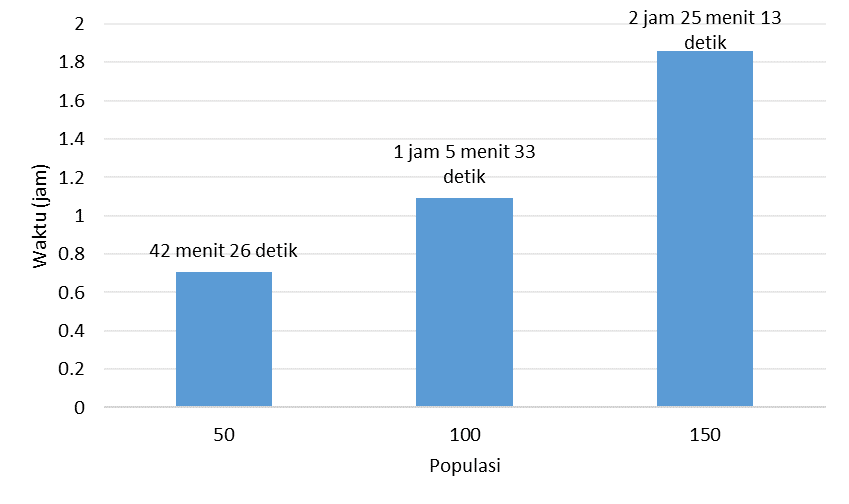
\includegraphics[width=0.6 \textwidth]{Diagram-pop-waktu}
			\caption{Grafik hubungan banyaknya populasi dengan waktu pengelompokan}
			\label{fig:graph:pop-time}
		\end{figure}
		
		Dapat disimpulkan dari diagram pada Gambar \ref{fig:graph:pop-time}, pada saat populasi berjumlah 100, waktu tempuh lebih lama 55\% dari saat populasi berjumlah 50. Pada saat populasi berjumlah 150, waktu tempuh 70\% lebih lama dibandingkan denga waktu pada saat populasi berjumlah 100. Kompleksitas algoritma genetika tidaklah linear sehingga menyebabkan kenaikan waktunya juga tidak linear. Selain itu, semakin banyak populasi maka calon solusi semakin banyak pula. Hal ini menyebabkan GA lebih sulit mencapai konvergen.
		
		\begin{figure}[H]
			\centering
			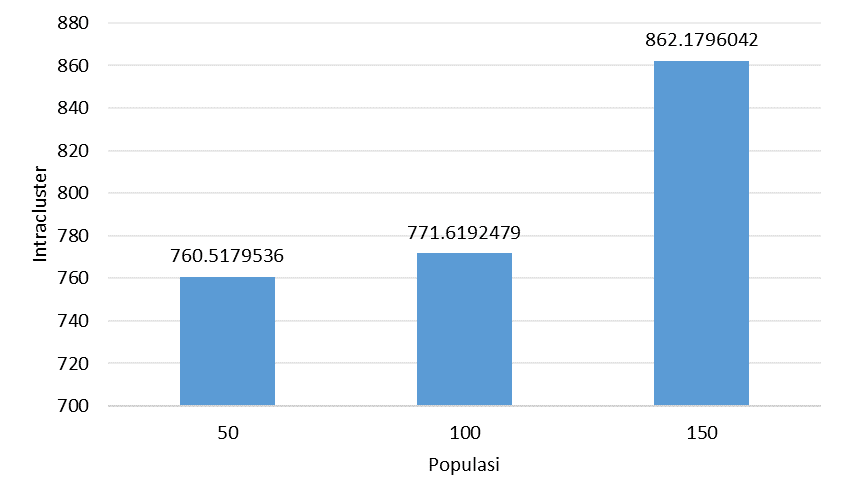
\includegraphics[width=0.6 \textwidth]{Diagram-pop-intracluster}
			\caption{Diagram hubungan banyaknya populasi dengan \textit{intracluster similarity}}
			\label{fig:graph:pop-intra}
		\end{figure}
		
		Dapat disimpulkan dari diagram pada Gambar \ref{fig:graph:pop-intra}, kenaikan populasi juga mempengaruhi kenaikan \textit{intracluster similarity}. \textit{Intracluster similarity} pada saat populasi berjumlah 100 lebih besar 1\% dibandingkan dengan \textit{intracluster similarity} pada saat populasi berjumlah 50. Sedangkan \textit{intracluster similarity} pada saat populasi berjumlah 150 lebih besar 11\% dibandingkan dengan \textit{intracluster similarity} pada saat populasi berjumlah 100. Hal ini dikarenakan dengan populasi yang lebih banyak maka kemungkinan untuk mendapat solusi yang lebih baik semakin besar.
		\begin{figure}[H]
			\centering
			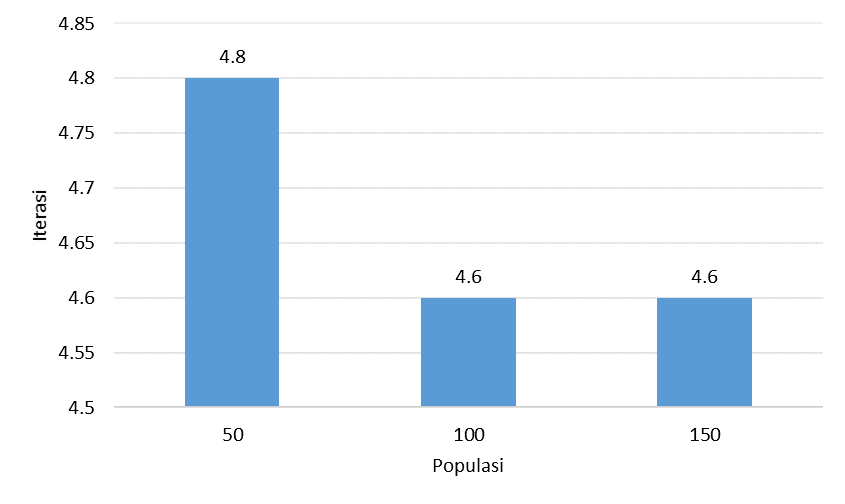
\includegraphics[width=0.6 \textwidth]{Diagram-pop-iterasi}
			\caption{Diagram hubungan banyaknya populasi dengan banyaknya iterasi}
			\label{fig:graph:pop-iteration}
		\end{figure}
		
		Dapat disimpulkan dari diagram pada Gambar \ref{fig:graph:pop-iteration}, kenaikan populasi tidak mempengaruhi banyaknya iterasi yang dilakukan dalam mencapai konvergen. Rata-rata banyaknya iterasi untuk populasi berjumlah 50, 100, dan 150 tidak memiliki perbedaan yang begitu signifikan.
		
		\begin{figure}[H]
			\centering
			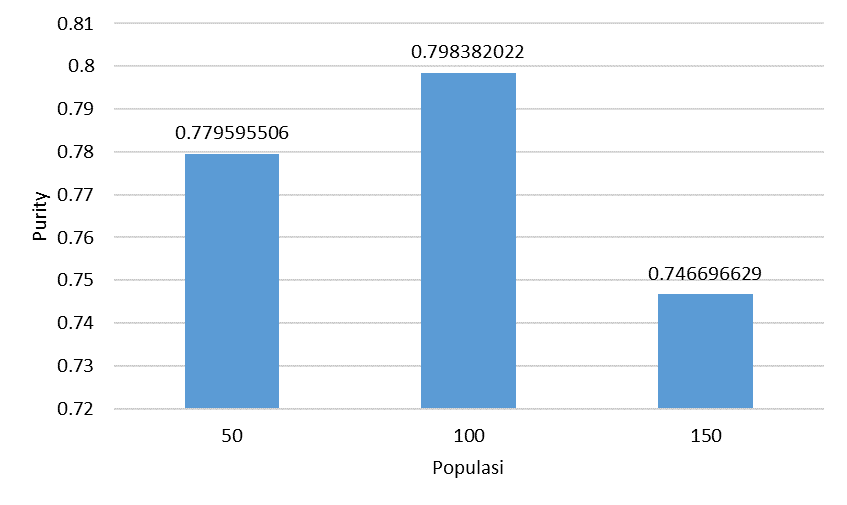
\includegraphics[width=0.6 \textwidth]{Diagram-pop-purity}
			\caption{Diagram hubungan banyaknya populasi dengan nilai \textit{purity}}
			\label{fig:graph:pop-purity}
		\end{figure}
		
		Dapat disimpulkan dari diagram pada Gambar \ref{fig:graph:pop-purity}, kenaikan populasi juga tidak mempengaruhi nilai \textit{purity} sama seperti banyaknya iterasi. Berdasarkan nilai \textit{purity}, maka hasil terbaik diperoleh dengan populasi sebanyak 100 individu. Nilai \textit{purity} pada saat populasi berjumlah 100 lebih besar 2\% dibandingkan dengan pada saat populasi berjumlah 50 dan 7\% lebih besar dibandingkan dengan pada saat populasi berjumlah 150.
		
		\item Metode pembobotan:
		\begin{table}[H]
			\centering
			\caption{Rata-rata hasil pengelompokan dengan variasi variabel metode pembobotan}
			\begin{tabular}{|l|l|l|l|l|} \hline
				Bobot & Waktu (jam) & \textit{Intracluster} & Iterasi& \textit{Purity} \\ \hline
				TF-IDF    & 1.092666667 & 771.6192479 & 4.6 & 0.798382022 \\ \hline
				Frekuensi & 2.733222222 & 1750.874933 & 7   & 0.571325843 \\ \hline
			\end{tabular}
			\label{tbl:exp-weight}
		\end{table}
		
		Berdasarkan Tabel \ref{tbl:exp-weight}, dibentuk empat buah diagram (Gambar \ref{fig:graph:weight-time} - \ref{fig:graph:weight-purity}) untuk menunjukan hubungan antara metode pembobotan dengan keempat variabel terikat.
		
		\begin{figure}[H]
			\centering
			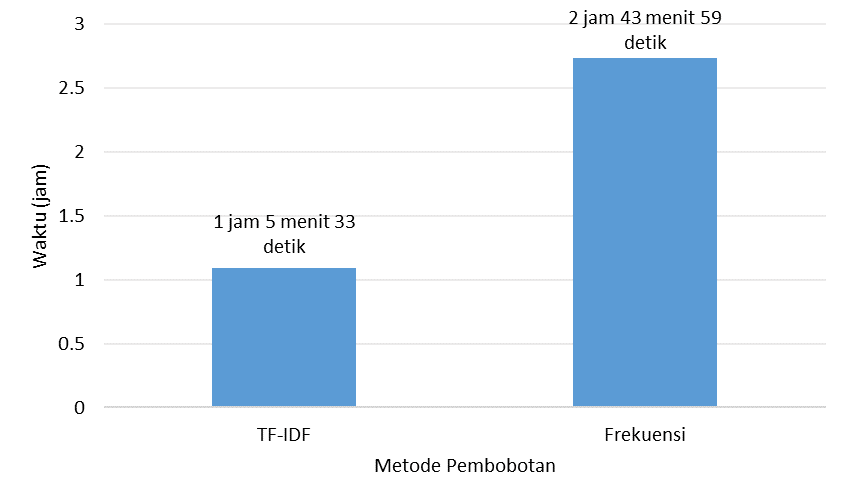
\includegraphics[width=0.6 \textwidth]{Diagram-bobot-waktu}
			\caption{Diagram hubungan metode pembobotan dengan waktu pengelompokan}
			\label{fig:graph:weight-time}
		\end{figure}
		
		Berdasarkan diagram pada Gambar \ref{fig:graph:weight-time}, waktu yang diperlukan untuk pengelompokan menggunakan bobot TF-IDF jauh lebih cepat hingga 167\% dibandingan dengan menggunakan bobot frekuensi. Hal ini kemungkinan memiliki kaitan dengan banyaknya iterasi yang terjadi selama proses pengelompokan.
		
		\begin{figure}[H]
			\centering
			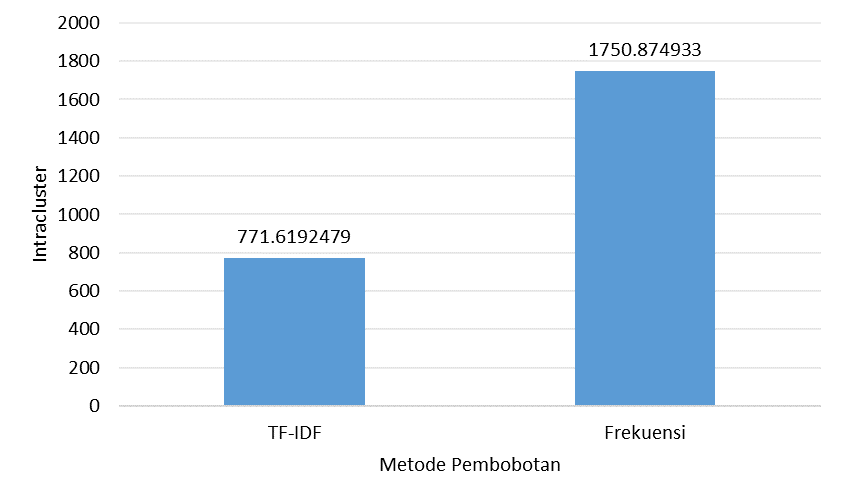
\includegraphics[width=0.6 \textwidth]{Diagram-bobot-intracluster}
			\caption{Diagram hubungan metode pembobotan dengan \textit{intracluster similarity}}
			\label{fig:graph:weight-intra}
		\end{figure}
		
		Berdasarkan diagram pada Gambar \ref{fig:graph:weight-intra}, \textit{intracluster similarity} yang dihasilkan menggunakan bobot TF-IDF hanya 44\% dari \textit{intracluster similarity} yang dihasilkan apabila menggunakan bobot frekuensi. Hal ini terjadi karena bobot frekuensi dari suatu dokumen pasti lebih besar nilainya dibandingkan dengan bobot TF-IDF.
		
		\begin{figure}[H]
			\centering
			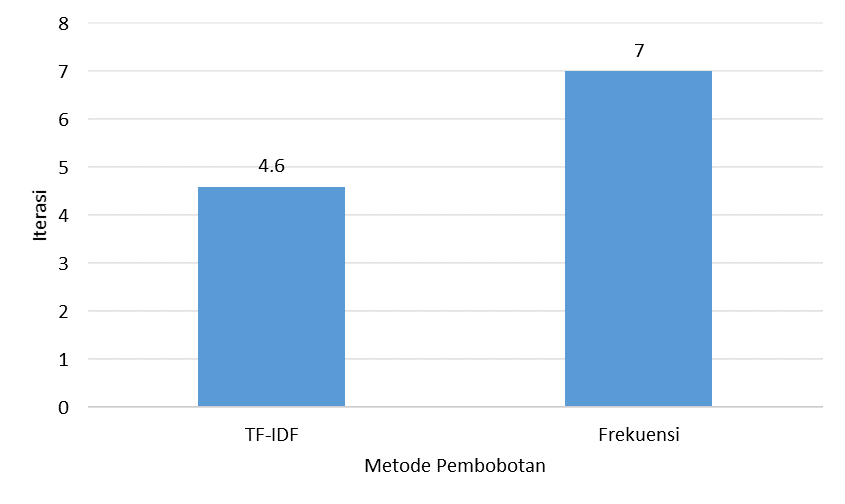
\includegraphics[width=0.6 \textwidth]{Diagram-bobot-iterasi}
			\caption{Diagram hubungan metode pembobotan dengan banyaknya iterasi}
			\label{fig:graph:weight-iteration}
		\end{figure}
		
		Berdasarkan diagram pada Gambar \ref{fig:graph:weight-iteration}, banyaknya iterasi yang dilakukan 52\% lebih banyak apabila menggunakan bobot frekuensi dibandingkan dengan menggunakan bobot TF-IDF.
		
		\begin{figure}[H]
			\centering
			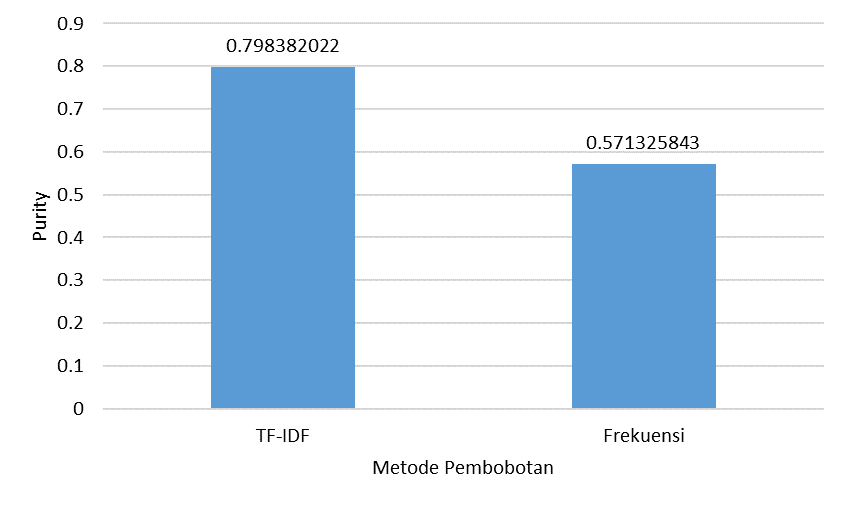
\includegraphics[width=0.6 \textwidth]{Diagram-bobot-purity}
			\caption{Diagram hubungan metode pembobotan dengan nilai \textit{purity}}
			\label{fig:graph:weight-purity}
		\end{figure}
		
		Berdasarkan diagram pada Gambar \ref{fig:graph:weight-purity}, nilai \textit{purity} yang didapatkan apabila menggunakan bobot TF-IDF 40\% lebih besar apabila dibandingkan dengan menggunakan bobot frekuensi. Hal ini terjadi karena dengan menggunakan bobot TF-IDF, representasi dokumen menjadi lebih akurat. Perhitungan bobot menggunakan TF-IDF tidak hanya ditentukan berdasarkan apa yang ada di dalam dokumen itu saja (lokal), namun juga mempertimbangkan faktor frekuensi dokumen secara global (Subbab \ref{sub:tf-idf}).
		
		\item Probabilitas mutasi:
		\begin{table}[H]
			\centering
			\caption{Rata-rata hasil pengelompokan dengan variasi variabel probabilitas mutasi}
			\begin{tabular}{|l|l|l|l|l|} \hline
				Probabilitas mutasi & Waktu (jam) & \textit{Intracluster} & Iterasi& \textit{Purity} \\ \hline
				0    & 1.650722222 & 1105.863837 & 5.2 & 0.632359551 \\ \hline
				0.05 & 1.092666667 & 771.6192479 & 4.6 & 0.798382022 \\ \hline
				0.25 & 1.566277778 & 1290.371505 & 5   & 0.437123596 \\ \hline
			\end{tabular}
			\label{tbl:exp-mutation}
		\end{table}
		
		Berdasarkan Tabel \ref{tbl:exp-mutation}, dibentuk empat buah diagram (Gambar \ref{fig:graph:mutation-time} - \ref{fig:graph:mutation-purity}) untuk menunjukan hubungan antara probabilitas mutasi dengan keempat variabel terikat.
		
		\begin{figure}[H]
			\centering
			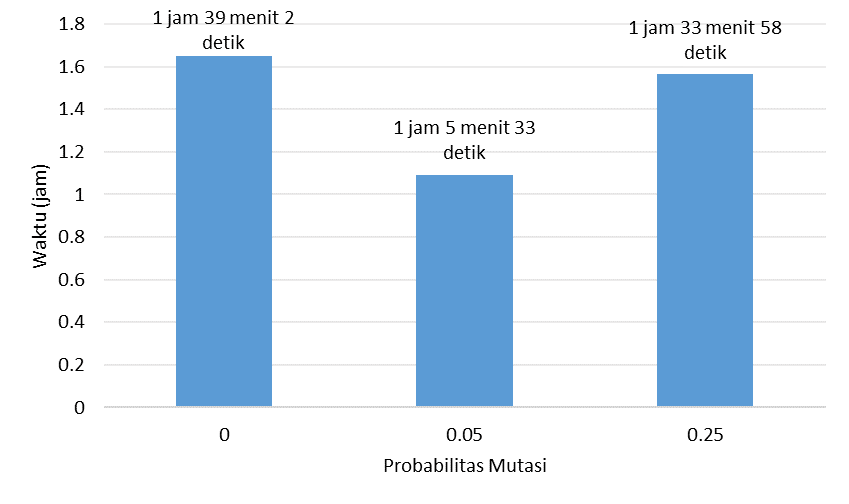
\includegraphics[width=0.6 \textwidth]{Diagram-mutation-waktu}
			\caption{Diagram hubungan probabilitas mutasi dengan waktu pengelompokan}
			\label{fig:graph:mutation-time}
		\end{figure}
		
		Dapat disimpulkan dari diagram pada Gambar \ref{fig:graph:mutation-time}, waktu tempuh paling cepat didapatkan dengan menggunakan probabilitas mutasi 0.05. Apabila probabilitas mutasi bernilai 0, maka mutasi tidak pernah terjadi sehingga GA lebih sulit mencapai konvergen. Hal ini menyebabkan waktu yang dibutuhkan untuk mencapai konvergen lebih lama. Apabila probabilitas mutasi bernilai 0.25, mutasi terjadi terlalu sering sehingga proses pencarian menjadi kurang terarah seperti yang telah dijelaskan pada Subbab \ref{sub:mutation}.
		
		\begin{figure}[H]
			\centering
			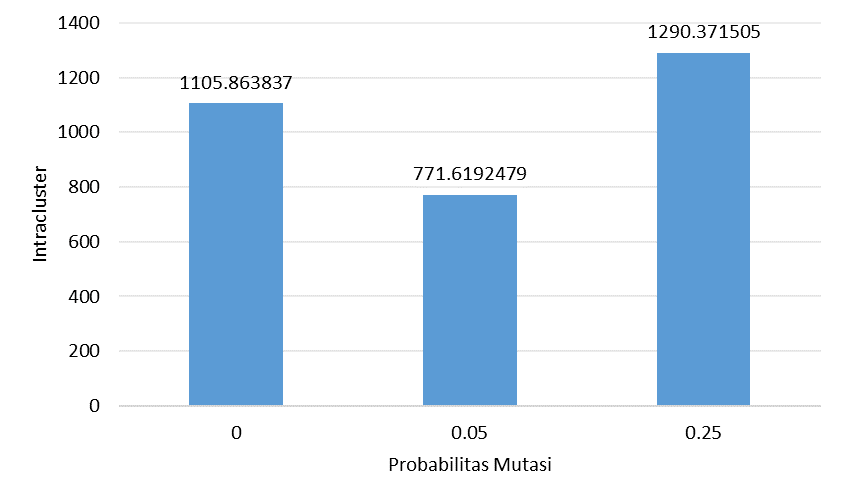
\includegraphics[width=0.6 \textwidth]{Diagram-mutation-intracluster}
			\caption{Diagram hubungan probabilitas mutasi dengan \textit{intracluster similarity}}
			\label{fig:graph:mutation-intra}
		\end{figure}
		
		Berdasarkan \textit{intracluster similarity} pada diagram dalam Gambar  \ref{fig:graph:mutation-intra}, hasil pengelompokan dengan probabilitas mutasi 0 lebih baik 43\% dari hasil menggunakan probabilitas mutasi 0.05. Hasil menggunakan probabilitas mutasi 0.25 juga lebih baik 67\% dibandingkan dengan menggunakan probabilitas mutasi 0.05.
		
		\begin{figure}[H]
			\centering
			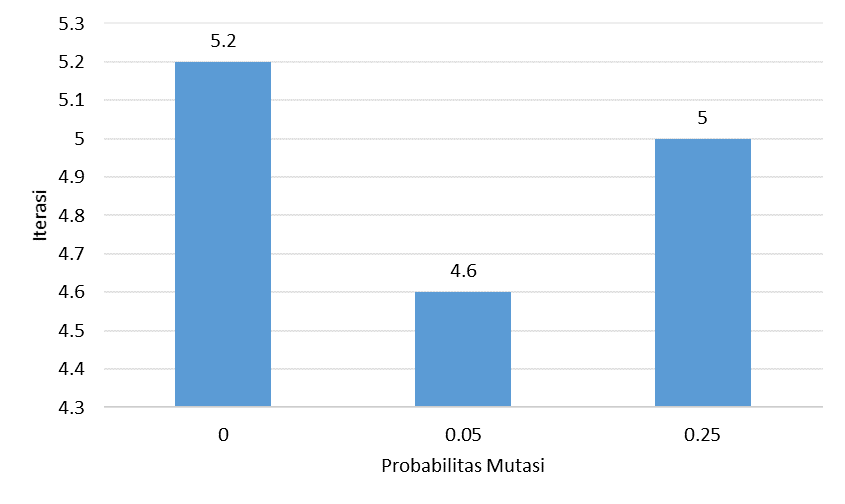
\includegraphics[width=0.6 \textwidth]{Diagram-mutation-iterasi}
			\caption{Diagram hubungan probabilitas mutasi dengan banyaknya iterasi}
			\label{fig:graph:mutation-iteration}
		\end{figure}
		
		Dapat disimpulkan dari diagram pada Gambar \ref{fig:graph:mutation-iteration}, jumlah iterasi paling sedikit didapatkan dengan menggunakan probabilitas mutasi 0.05. Sama dengan waktu tempuh, apabila probabilitas mutasi bernilai 0, maka mutasi tidak pernah terjadi sehingga GA lebih sulit mencapai konvergen. Hal ini menyebabkan jumlah iterasi yang dibutuhkan untuk mencapai konvergen lebih banyak. Apabila mutasi terjadi terlalu sering (pada kasus ini dengan probabilitas 0.25), maka GA juga sulit mencapai konvergen karena proses pencariannya menjadi tidak terarah.
		
		\begin{figure}[H]
			\centering
			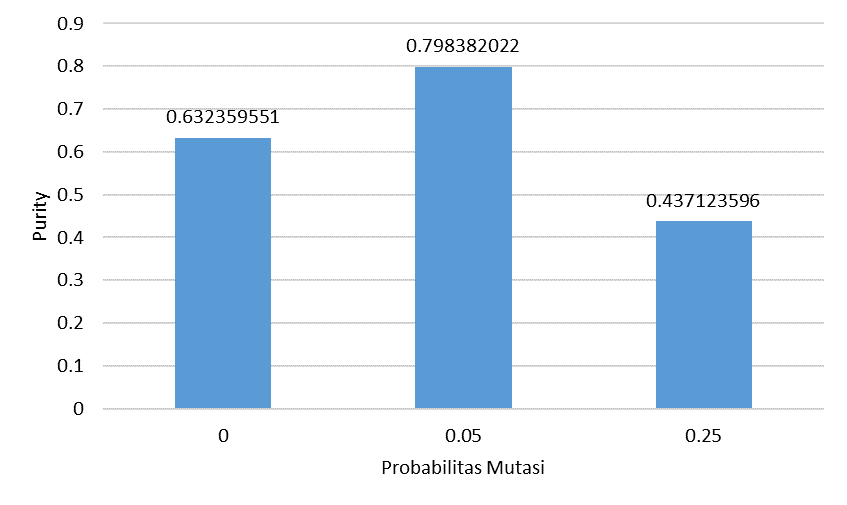
\includegraphics[width=0.6 \textwidth]{Diagram-mutation-purity}
			\caption{Diagram hubungan probabilitas mutasi dengan nilai \textit{purity}}
			\label{fig:graph:mutation-purity}
		\end{figure}
		
		Berdasarkan nilai \textit{purity} pada diagram dalam Gambar \ref{fig:graph:mutation-purity}, hasil terbaik didapatkan dengan menggunakan probabilitas mutasi 0.05. Nilai \textit{purity} dengan menggunakan probabilitas mutasi 0.05 lebih baik 26\% dibandingkan dengan menggunakan probabilitas mutasi 0 dan lebih baik 82\% dibandingkan menggunakan probabilitas mutasi 0.25.
		
		\newpage
		\item Individu elitisme:
		\begin{table}[H]
			\centering
			\caption{Rata-rata hasil pengelompokan dengan variasi variabel individu elitisme}
			\begin{tabular}{|l|l|l|l|l|} \hline
				Individu elitisme & Waktu (jam) & \textit{Intracluster} & Iterasi & \textit{Purity} \\ \hline
				0 & 5.963388889 & 679.7977532 & 15  & 0.826247191 \\ \hline
				1 & 1.092666667 & 771.6192479 & 4.6 & 0.798382022 \\ \hline
				5 & 2.081777778 & 1215.335516 & 6   & 0.527101124 \\ \hline
			\end{tabular}
			\label{tbl:exp-elitism}
		\end{table}
		
		Karena keterbatasan waktu, untuk eksperimen tanpa individu elitisme (individu elitisme=0), banyaknya iterasi maksimum hanya dibatasi sampai dengan 15 iterasi saja. Berdasarkan Tabel \ref{tbl:exp-elitism}, dibentuk empat buah diagram (Gambar \ref{fig:graph:elite-time} - \ref{fig:graph:elite-purity}) untuk menunjukan hubungan antara metode pembobotan dengan keempat variabel terikat.
		
		\begin{figure}[H]
			\centering
			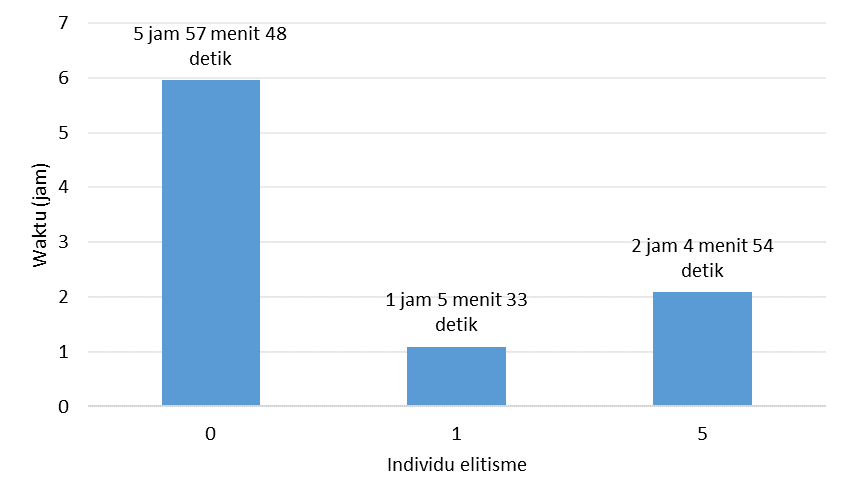
\includegraphics[width=0.6 \textwidth]{Diagram-elit-waktu}
			\caption{Diagram hubungan individu elitisme dengan waktu pengelompokan}
			\label{fig:graph:elite-time}
		\end{figure}
		
		Dapat disimpulkan dari diagram pada Gambar \ref{fig:graph:elite-time}, waktu tempuh pada saat individu elitisme berjumlah 1 paling sebentar apabila dibandingkan dengan pada saat individu elitisme berjumlah 0 atau 5. Waktu terlama dicapai pada saat tidak ada individu elitisme. Hal ini dikarenakan algoritma genetika sulit mencapai konvergen tanpa bantuan elitisme. Apabila jumlah individu elitisme terlalu banyak (pada eksperimen ini berjumlah 5), calon solusi dengan nilai \textit{fitness} tinggi lebih banyak sehingga diperlukan waktu yang lebih lama untuk dapat mencapai konvergen.
		
		\begin{figure}[H]
			\centering
			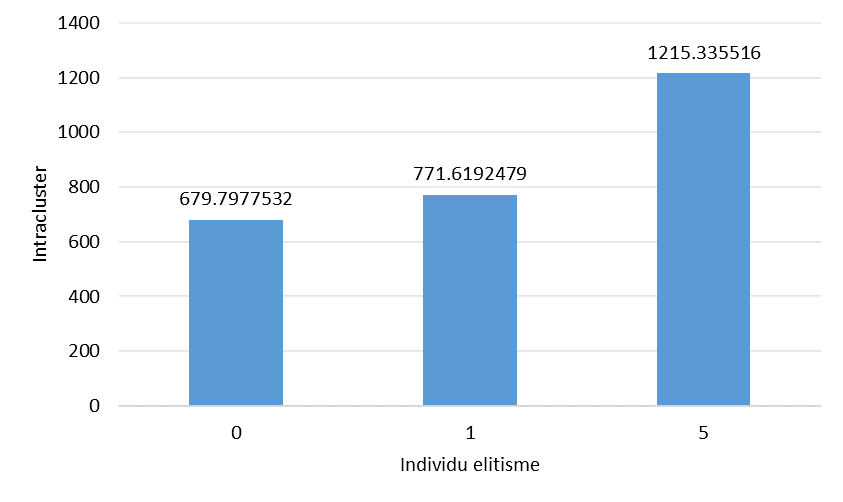
\includegraphics[width=0.6 \textwidth]{Diagram-elit-intracluster}
			\caption{Diagram hubungan individu elitisme dengan \textit{intracluster similarity}}
			\label{fig:graph:elite-intra}
		\end{figure}
		
		Dapat disimpulkan dari diagram pada Gambar \ref{fig:graph:elite-intra}, semakin banyak jumlah individu elitisme, maka semakin banyak individu dengan nilai \textit{fitness} tinggi yang dipertahankan sehingga memperbesar kemungkinan untuk menghasilkan individu dengan nilai \textit{fitness} yang lebih tinggi lagi.
		
		\begin{figure}[H]
			\centering
			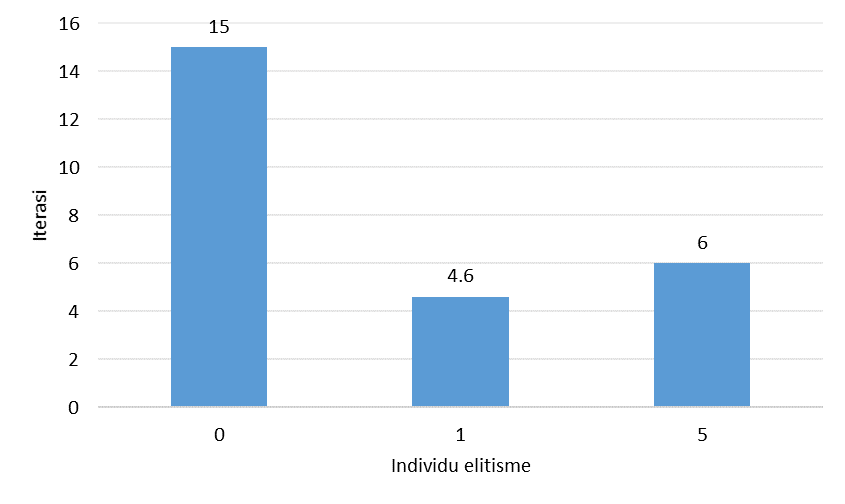
\includegraphics[width=0.6 \textwidth]{Diagram-elit-iterasi}
			\caption{Diagram hubungan individu elitisme dengan banyaknya iterasi}
			\label{fig:graph:elite-iteration}
		\end{figure}
		
		Sama halnya dengan waktu, berdasarkan diagram pada Gambar \ref{fig:graph:elite-iteration}, banyaknya iterasi pada saat proses pengelompokan terjadi tanpa individu elitisme lebih banyak (dalam eksperimen ini mencapai batas maksimum iterasi). Hal ini terjadi karena lebih sulit untuk mencapai konvergen tanpa ada bantuan dari elitisme. Banyaknya iterasi paling minimum dicapai dengan 1 individu elitisme. Proses pengelompokan dengan banyak individu elitisme hanya memperlambat proses pengelompokan karena kandidat solusi dengan nilai \textit{fitness} tinggi menjadi lebih banyak dan terus dipertahankan dalam populasi sehingga memperlambat GA dalam mencapai konvergen.
		
		\begin{figure}[H]
			\centering
			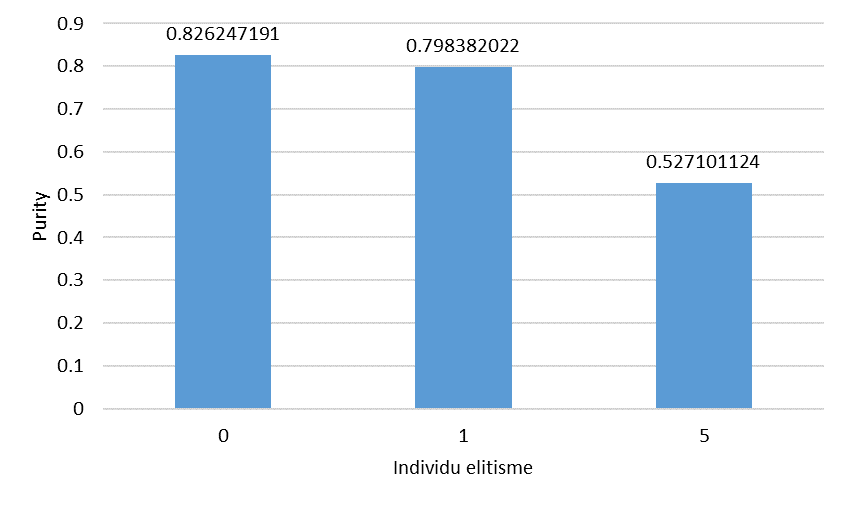
\includegraphics[width=0.6 \textwidth]{Diagram-elit-purity}
			\caption{Diagram hubungan individu elitisme dengan nilai \textit{purity}}
			\label{fig:graph:elite-purity}
		\end{figure}
		
		Dapat disimpulkan dari diagram pada Gambar \ref{fig:graph:elite-purity}, nilai \textit{purity} pada saat individu elitisme berjumlah 0 lebih besar 3\% dibandingkan dengan pada saat individu elitisme berjumlah 1. Hal ini mungkin disebabkan oleh banyaknya iterasi yang ditempuh pada saat individu elitisme berjumlah 0 jauh lebih banyak dibandingkan dengan pada saat individu elitisme berjumlah 1. Dengan jumlah iterasi yang lebih banyak, maka hasilnya semakin baik. Nilai \textit{purity} pada saat individu elitisme berjumlah 1 lebih besar 51\% dibandingkan dengan pada saat individu elitisme berjumlah 5. Hal ini mungkin terjadi karena individu yang dibawa pada saat proses elitisme mungkin saja individu dengan nilai \textit{fitness} rendah. Semakin banyak individu yang dibawa ke generasi selanjutnya dalam elitisme, maka semakin besar kemungkinan membawa individu dengan nilai \textit{fitness} rendah.
\end{enumerate}

\section{Eksperimen \textit{K-Means}}
Sebagai perbandingan terhadap pengelompokan menggunakan algoritma genetika, maka dibuat pula eksperimen menggunakan algoritma \textit{K-means}. Seperti yang telah dijelaskan pada Subbab \ref{sub:ui-kmeans}, pada penelitian ini \textit{K-means} hanya memiliki tiga buah parameter. Hanya satu di antara ketiga parameter tersebut yang dapat dijadikan variabel bebas karena alasan yang sama dengan yang telah dijelaskan pada Subbab \ref{sec:exp-scenario}. Eksperimen menggunakan algoritma \textit{K-means} hanya dilakukan menggunakan dua variasi yaitu dengan metode pembobotan TF-IDF dan Frekuensi. Namun dalam eksperimen pada penelitian ini, hanya variasi menggunakan bobot TF-IDF yang diuji. Hasil dari eksperimen menggunakan algoritma \textit{K-means} ini kemudian dibandingkan dengan kasus uji ideal pada algoritma genetika. Berbeda dari pengujian menggunakan algoritma genetika, pengujian menggunakan \textit{K-means} dilakukan sebanyak 10 kali tiap variasi. Hasil eksperimen menggunakan algoritma \textit{K-means} dijelaskan dalam Tabel \ref{tbl:exp-kmeans}.

\begin{table}[H]
	\centering
	\caption{Rata-rata hasil pengelompokan dengan menggunakan algoritma \textit{K-means}}
	\begin{tabular}{|l|l|l|l|l|} \hline
		Algoritma & Waktu (jam) & \textit{Intracluster} & Iterasi& \textit{Purity} \\ \hline
		GA      & 1.092666667 & 771.6192479 & 4.6  & 0.798382022 \\ \hline
		\textit{K-means} & 0.024472222 & 831.5881861 & 11.5 & 0.51191103 \\ \hline
	\end{tabular}
	\label{tbl:exp-kmeans}
\end{table}

Berdasarkan Tabel \ref{tbl:exp-kmeans}, dibentuk empat diagram pada Gambar \ref{fig:graph:kmeans-time} - \ref{fig:graph:kmeans-purity} untuk menjelaskan perbandingan antara algoritma genetika dengan algoritma \textit{K-means} berdasarkan keempat variabel terikat.

\begin{figure}[H]
	\centering
	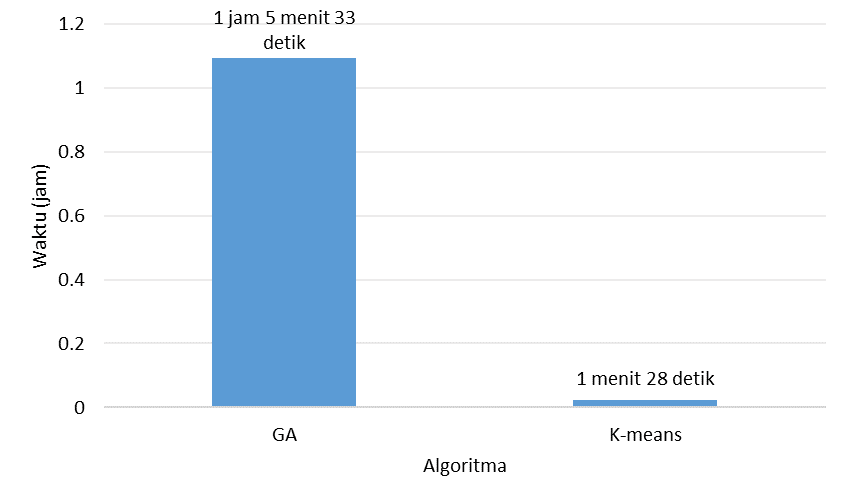
\includegraphics[width=0.6 \textwidth]{Diagram-kmeans-waktu}
	\caption{Diagram hubungan algoritma dengan waktu tempuh}
	\label{fig:graph:kmeans-time}
\end{figure}

Berdasarkan diagram pada Gambar \ref{fig:graph:kmeans-time}, waktu yang dibutuhkan algoritma genetika lebih banyak sekitar 4365\% dibandingkan dengan algoritma \textit{K-means}. Hal ini dikarenakan proses komputasi yang dilakukan pada algoritma genetika jauh lebih banyak dan kompleks dibandingkan dengan algoritma \textit{K-means}.

\begin{figure}[H]
	\centering
	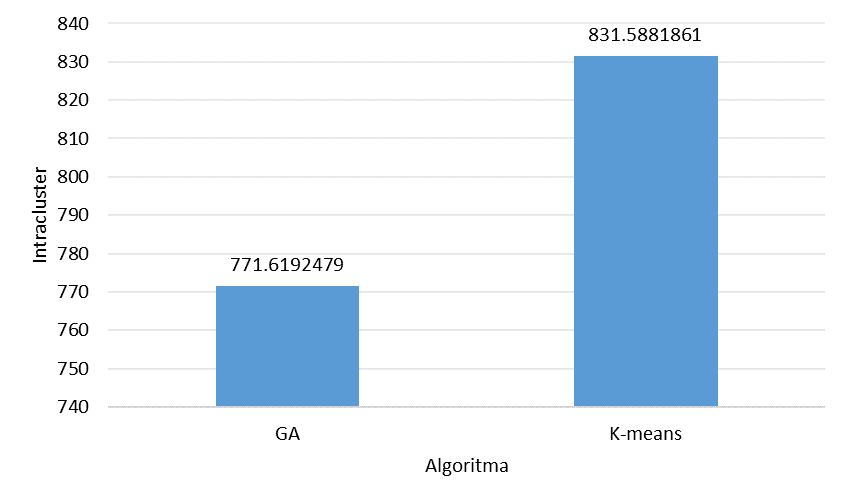
\includegraphics[width=0.6 \textwidth]{Diagram-kmeans-intracluster}
	\caption{Diagram hubungan algoritma dengan \textit{intracluster similarity}}
	\label{fig:graph:kmeans-intra}
\end{figure}

Berdasarkan diagram pada Gambar \ref{fig:graph:kmeans-intra}, nilai \textit{intracluster similarity} pada algoritma \textit{K-means} lebih besar 7\% daripada algoritma genetika.

\begin{figure}[H]
	\centering
	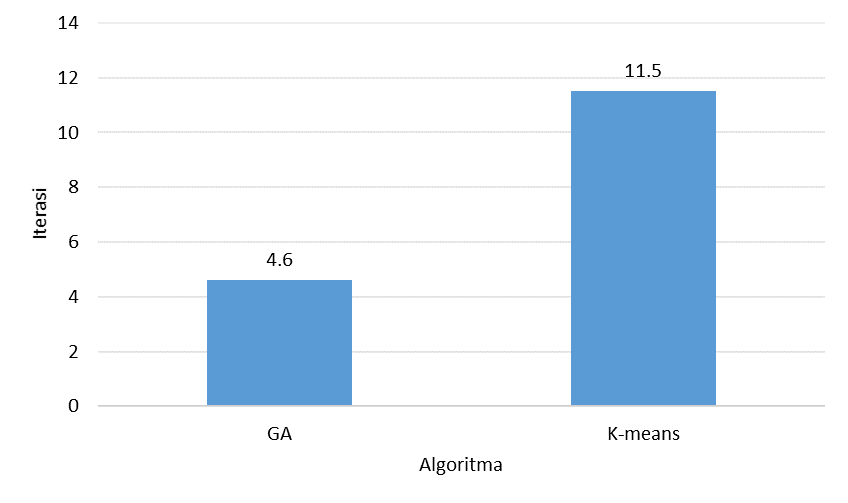
\includegraphics[width=0.6 \textwidth]{Diagram-kmeans-iterasi}
	\caption{Diagram hubungan algoritma dengan banyaknya iterasi}
	\label{fig:graph:kmeans-iteration}
\end{figure}

Berdasarkan diagram pada Gambar \ref{fig:graph:kmeans-iteration}, jumlah iterasi dengan menggunakan algoritma \textit{K-means} lebih banyak 150\% daripada algoritma genetika. Namun berdasarkan diagram pada Gambar \ref{fig:graph:kmeans-time}, waktu yang ditempuh \textit{K-means} lebih sebentar dibandingkan dengan algoritma genetika. Hal ini terjadi karena waktu yang diperlukan untuk menempuh satu iterasi pada \textit{K-means} jauh lebih kecil dibandingkan dengan waktu yang diperlukan untuk menempuh satu iterasi pada algoritma genetika.

\begin{figure}[H]
	\centering
	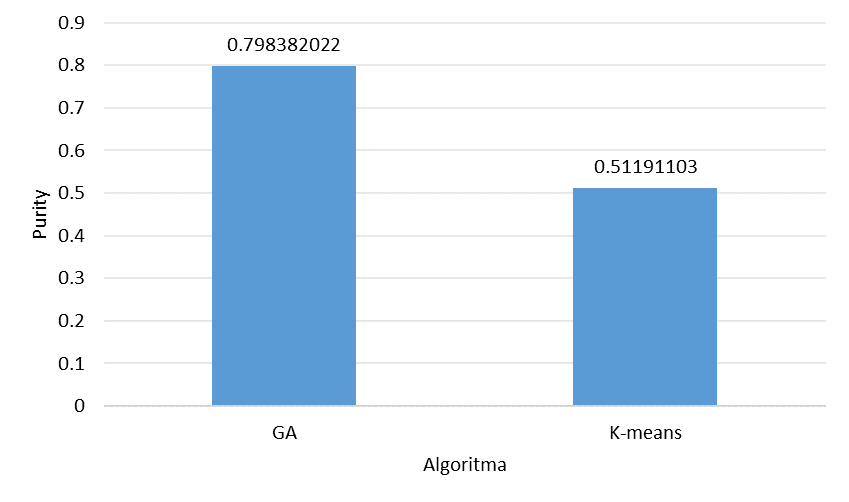
\includegraphics[width=0.6 \textwidth]{Diagram-kmeans-purity}
	\caption{Diagram hubungan algoritma dengan nilai \textit{purity}}
	\label{fig:graph:kmeans-purity}
\end{figure}

Berdasarkan diagram pada Gambar \ref{fig:graph:kmeans-purity}, nilai \textit{purity} algoritma genetika lebih besar 56\% dibandingkan dengan nilai \textit{purity} menggunakan algoritma \textit{K-means}.

\section{Analisis Hasil Eksperimen}
Berikut merupakan hasil analisis berdasarkan hasil eksperimen yang telah dilakukan.

\begin{enumerate}
	\item \textit{Intracluster similarity} belum dapat menentukan apakah hasil dari suatu pengelompokan sudah baik atau belum. Berdasarkan hasil eksperimen, nilai \textit{intracluster} similarity tidak berbanding lurus dengan nilai \textit{purity}. Salah satu kemungkinannya adalah karena semakin jauh jarak suatu anggota \textit{cluster} dari \textit{centroid}, maka nilai \textit{intracluster similarity} semakin kecil. Nilai \textit{purity} merupakan suatu nilai biner sehingga sejauh apapun suatu anggota \textit{cluster} dari \textit{centroid}, objek tersebut tetap merupakan anggota dari \textit{cluster}. Kemungkinan yang terjadi adalah banyak objek yang jaraknya cukup jauh dari \textit{centroid} namun tetap merupakan bagian dari \textit{cluster} tersebut karena jarak ke \textit{centroid} lain lebih jauh. Hal ini yang dapat menyebabkan suatu hasil pengelompokan memiliki \textit{intracluster similarity} bernilai kecil sedangkan \textit{purity} bernilai besar atau sebaliknya.
	\item Algoritma genetika lebih baik 56\% menurut nilai \textit{purity} (Gambar \ref{fig:graph:kmeans-purity}). Namun, kekurangan dari algoritma genetika adalah waktu pemrosesan yang jauh lebih lama dibandingkan dengan algoritma \textit{K-means}. 
	
	\item Untuk membandingkan antara algoritma \textit{K-means} dengan algoritma genetika, maka dilakukan operasi statistika dasar terhadap data hasil eksperimen (Tabel \ref{tbl:resKM} dan Tabel \ref{tbl:res1} pada Lampiran \ref{lamp:B}). Hasil perhitungan statistika dasar terhadap kedua tabel tersebut dijelaskan dalam Tabel \ref{tbl:stat-res}.
	
\begin{table}[H]
\caption{Hasil perhitungan statistika terhadap hasil eksperimen algoritma genetika dan \textit{K-means}}
\begin{tabular}{|l|l|l|l|l|l|}
\hline
\multicolumn{2}{|l|}{Algoritma}         & Rata-rata   & Standar Deviasi & Nilai Maksimum & Nilai Minimum \\ \hline
\multirow{2}{*}{GA}      & \textit{intracluster} & 771.6192479 & 18.93213605     & 781.7710303    & 733.7897158   \\ \cline{2-6} 
                         & \textit{purity}       & 0.798382022 & 0.01228077      & 0.820224719    & 0.78741573    \\ \hline
\multirow{2}{*}{\textit{K-means}} & \textit{intracluster} & 831.5881861 & 272.6741901     & 1383.188573    & 512.6894755   \\ \cline{2-6} 
                         & \textit{purity}       & 0.51191103  & 0.20861176      & 0.794606742    & 0.248153619   \\ \hline
\end{tabular}
\label{tbl:stat-res}
\end{table}
	
	Berdasarkan Tabel \ref{tbl:stat-res}, standar deviasi dari nilai \textit{intracluster} pada algoritma \textit{K-means} 1340\% lebih besar dibandingkan dengan algoritma genetika. Selain itu, standar deviasi dari nilai \textit{purity} pada algoritma \textit{K-means} 1599\% lebih besar dibandingkan dengan algoritma genetika. Standar deviasi yang bernilai besar pada algoritma \textit{K-means} membuktikan bahwa pesebaran data cukup luas. Hal ini juga didukung dengan jarak antara nilai maksimum dan minimum yang cukup jauh untuk nilai \textit{intracluster} maupun \textit{purity} pada algoritma \textit{K-means}. Pesebaran data yang meluas membuktikan bahwa hasil dari algoritma \textit{K-means} tidak stabil. Hal ini juga berarti bahwa algoritma \textit{K-means} sering terjebak pada \textit{local optimum}.
	
	Untuk algoritma genetika, standar deviasi untuk kedua variabel tidak begitu besar. Hal ini membuktikan bahwa pesebaran data pada algoritma genetika cukup sempit. Hal ini didukung dengan jarak antara nilai minimum dan maksimum untuk kedua variabel pada algoritma genetika tidak begitu jauh. Pesebaran data yang sempit membuktikan bahwa hasil dari algoritma genetika cukup stabil. Hal ini dapat membuktikan bahwa algoritma genetika lebih baik dalam mengatasi \textit{local optimum} dibandingkan dengan algoritma \textit{K-means}.
\end{enumerate}